\documentclass[twocolumn]{article}
\usepackage{array,url,kantlipsum}
\usepackage{geometry}
\usepackage[backend=biber,sorting=none]{biblatex}
\usepackage{booktabs}
\usepackage{float}

\bibliography{ref.bib}

 \geometry{
 a4paper,
 total={210mm,297mm},
 left=20mm,
 right=20mm,
 top=25mm,
 bottom=25mm,
 }
% \Mark is probably provided by spconf, that I don't have
\newcommand{\Mark}[1]{\textsuperscript{#1}}

\usepackage{siunitx}
\usepackage{amsmath}
\usepackage{fouriernc}
\usepackage{graphicx}
\usepackage[colorlinks=true]{hyperref}
\usepackage{subcaption}

\newcommand{\COtwo}{\textnormal{CO}_2}
\newcommand{\Otwo}{\textnormal{O}_2}
\newcommand{\CHfour}{\textnormal{CH}_4}
\newcommand{\Htwo}{\textnormal{H}_2}
\newcommand{\HtwoO}{\textnormal{H}_2\textnormal{O}}
\newcommand{\ud}{\operatorname{d}}

\begin{document}

\begin{titlepage}

  \vspace{5cm}

  \begin{center}
    {\Huge
    \textsc{Mars UPV Team}}
    
    \vspace{1cm}
    {\LARGE Technical Report 0001}
  \end{center}
 
  \vspace{0.5cm}
 
  \begin{center}
    \LARGE
    \textsc{Feasibility Study Of A Jet-pack System For Mars Operations}
  \end{center}

 
  \vspace{\fill}
  
  \begin{figure}[H]
    \centering
    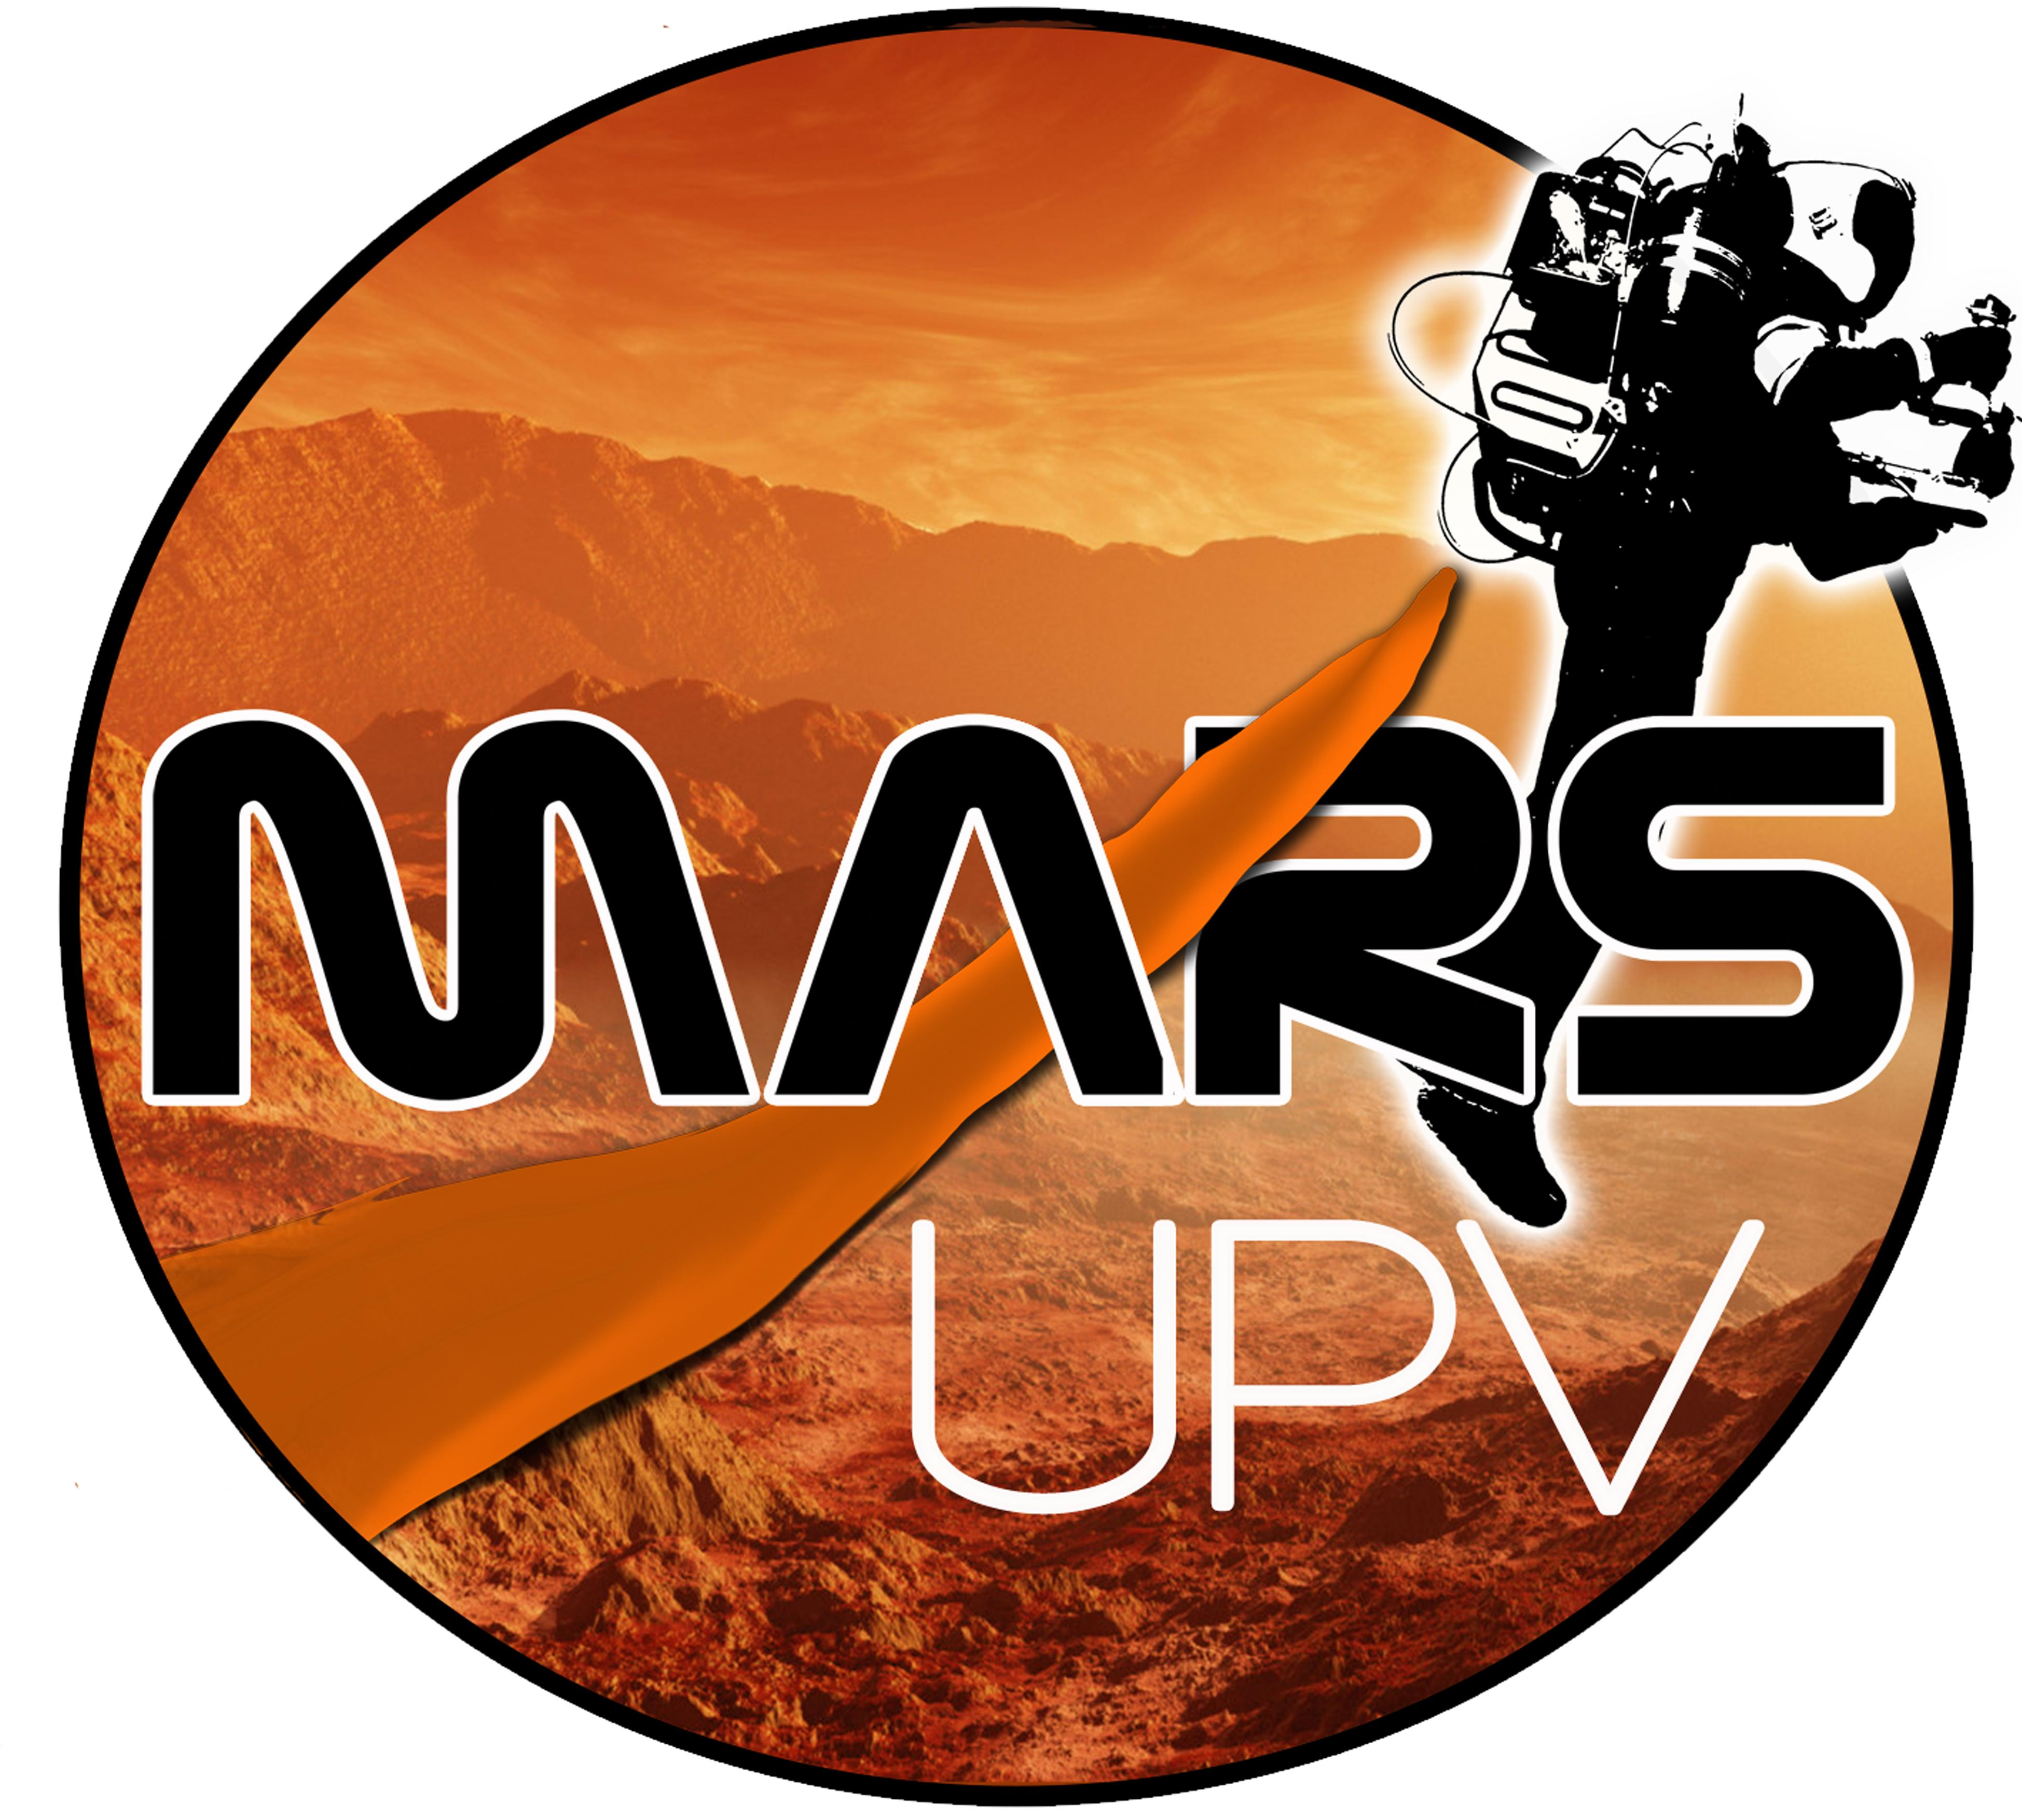
\includegraphics[width=12cm]{img/Logo_Mars_UPV_A3}
  \end{figure}

  \vspace{\fill}

  \begin{center}
     \Large Valencia, April 24, 2016
  \end{center}
  
  \vspace{1cm}
  
\end{titlepage}

\clearpage

\thispagestyle{empty}
\phantom{asd}

\clearpage

\setcounter{page}{1}

\twocolumn[{%
 \centering
 \LARGE \textbf{Feasibility Study Of A Jet-pack System For Mars Operations} 
\\[1.5em]
 \large \textit{Mars UPV Team, 2016}\\[1em]
 \normalsize
% \begin{tabular}{*{2}{>{\centering}p{.25\textwidth}}}
%  \Mark{1}Department1 & \Mark{2}Department2 \tabularnewline
%  School1 & School2  \tabularnewline
%  \url{email1} & \url{email2}
% \end{tabular}\\[3em] % some more space after the title part
}]

\begin{abstract}
From superhero movies to video-games we have tried to imagine an individual jet 
propulsion system to fly on our own. We have several attempts of this system 
over the world, but why don't we apply this technology to the exploration of 
Mars? In this paper we are going to develop the mathematical background of an 
hypothetical martian jet-pack design. 
\end{abstract}

\section{Introduction}
The exploration of Mars is now a priority to NASA. During the first phases of 
human settlement in Mars, the astronauts will need to do a lot of activities
outside of the habitats, including scientific, building and maintenance 
missions.

At this point, is where a jet-pack could be extremely advantageous. The 
development of this system will enable the astronaut to explore Mars as never 
has been done. The jet-pack allow the pilot to overcome obstacles such as 
mountains and rocks. Moreover, it permits the explorer to travel at higher 
speeds. The rocket engine proposed in this work burns liquid methane with 
liquid oxygen, as they are easily produced using on-site resources. An 
exoskeleton is used to reduce the weight burden in the astronaut, improving its 
force.

The modules needed to assembly the jet-pack and the different facilities needed 
to produce the propellant can be sent from Earth, but later developments might 
enable to build them directly from Mars resources.

\section{Propellant production}

As $\COtwo$ is extremely abundant in the Mars atmosphere, the 
Sabatier reaction is a clear candidate for producing methane fuel for the 
jet-pack. In this reaction, $\COtwo$ is mixed with 
$\Htwo$ in a reactor, producing $\CHfour$, water and heat:

\begin{equation}
  \COtwo + \CHfour \rightarrow \CHfour + 2 \HtwoO
  - \SI{165}{\kilo\joule\per\mol}
\end{equation}

Water can be recycled and electrolized to produce hydrogen and oxygen:

\begin{equation}
  \HtwoO + \SI{286}{\kilo\joule\per\mol} \rightarrow
  \Htwo + \cfrac{1}{2} \Otwo
\end{equation}

The waste heat of the Sabatier reaction can be used to heat up the electrolysis 
reactor, so its energy consumption can be reduced. In order to produce one mol 
of $\CHfour$, \SI{2}{\mol} of $\HtwoO$ have to be extracted from the ground. 
The water extraction can be easily performed if the soil contains high amounts 
of ice: ground fragments can be put into contact with pressurized atmosphere at 
moderate temperatures, so the water ice melts instead of sublimating, producing 
liquid water. Hydrogen trapped in rocks can be extracted using supercritical
$\COtwo$, trapping $\textnormal{C}$ in the ground and producing water. Using 
data from \cite{methanator}, a methanator producing \SI{10}{\kilogram} of 
propellant per day has an estimated weight of around \SI{500}{\kilogram}.

The energy budget for the methanator is estimated using a heat transfer 
efficiency of \SI{60}{\percent}, an electrolysis efficiency of 
\SI{60}{\percent},

typical solar cell efficiency as in the Opportunity Rover 
and 
assuming that an astronaut cleans the cells from dust 
\cite{opportunity_power,merlaunch}. In this case, 
\SI{692}{\watt\hour\per\square\metre} are produced per sol, and 
\SI{10.5}{\kilo\watt\hour} are needed per \si{\kilogram} of propellant, leading 
to slightly more than \SI{150}{\square\metre} to produce \SI{10}{\kilogram} of 
propellant per sol. Typical monocrystalline and polycrystalline solar panels 
weight between \SI{10}{\kilogram\per\square\metre} and 
\SI{20}{\kilogram\per\square\metre}, so between \SI{150}{\kilogram} and 
\SI{300}{\kilogram} will be needed. The modular nature of solar arrays ensures 
that they can be easily disassembled, transported and reassembled if they are 
needed elsewhere. Other options could be also used, such as a small nuclear 
reactor transported by a light truck, but the solar panels reduce the mission 
risks and are more easily replaceable.

This solution differs from other such as the ones proposed in 
\cite{mars_direct} in that, instead of using $\Htwo$ sent from Earth, it uses 
only resources from Mars.

\section{Mars region selection}

Comparing different regions of Mars by studying different maps of Mars' relief, 
the composition of the soil in Mars, the percentage of hydrogen in the first 
meter of Mars's soil and the location of Mars' equator, we have decided to 
perform our mission in the region called `Arabia Terra'. 

'Arabia Terra' is a region that is located at 0 longitude and just above the 
equator, what we where looking for. As we can see in the upper part of 
\autoref{fig:arabia_terra}, the relief in the selected region is almost plane 
and constant over all the surface. Also, the reduced height ensures a 
relatively high atmospheric pressure, so it can be more easily used. 
Taking a look at the bottom part of \autoref{fig:arabia_terra}, the percentage 
of Hydrogen concentration in this region is high enough to ensure a supply of 
$\Htwo$ for the duration of the mission. This figures have been produced by 
modifying the works from \cite{mars_elevation_and_boundaries} and 
\cite{water_on_mars}.

\begin{figure*}
  \centering
  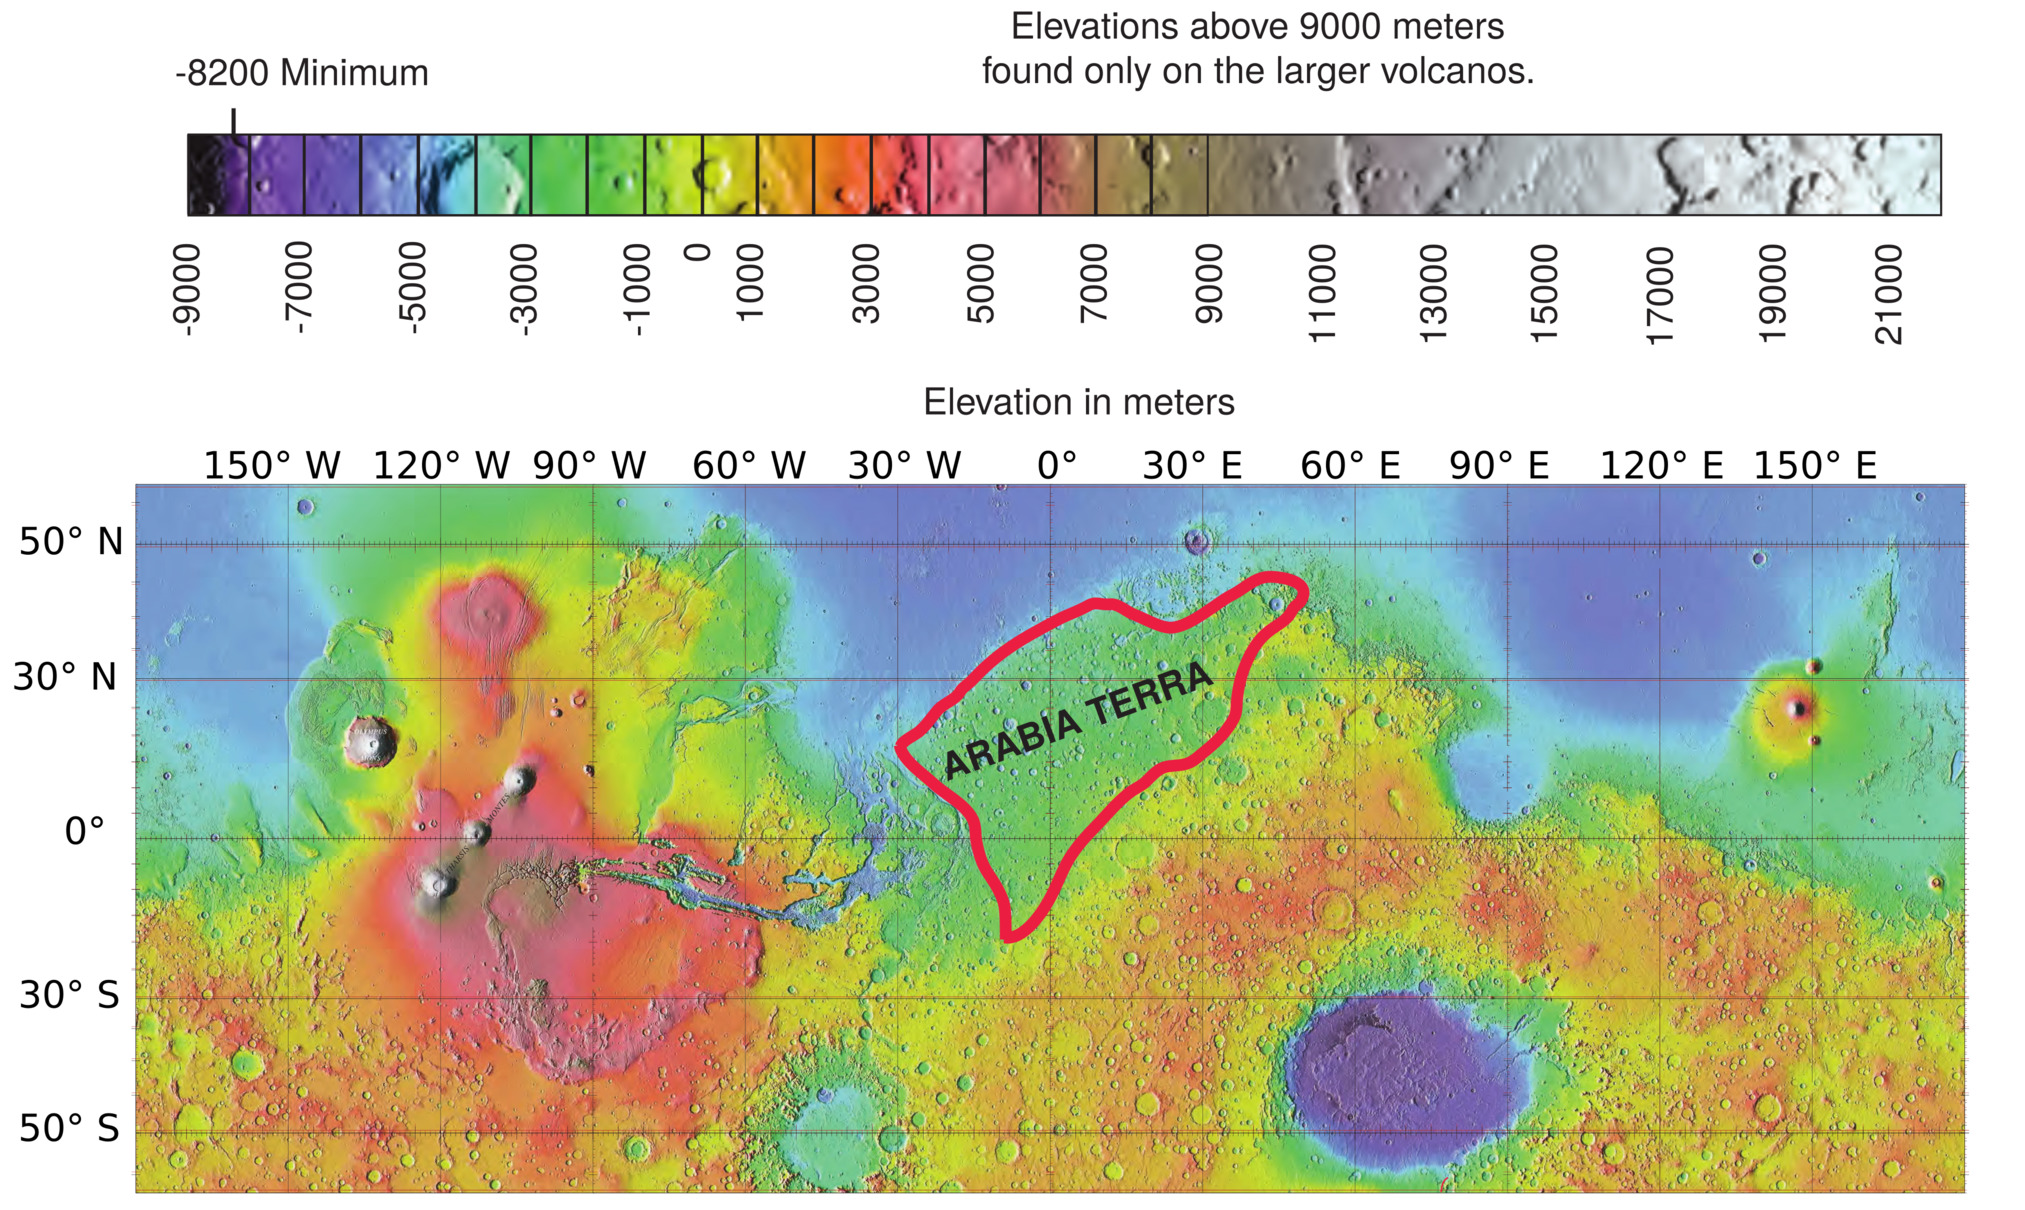
\includegraphics[width=\textwidth]{img/mola_regional_boundaries_2}
  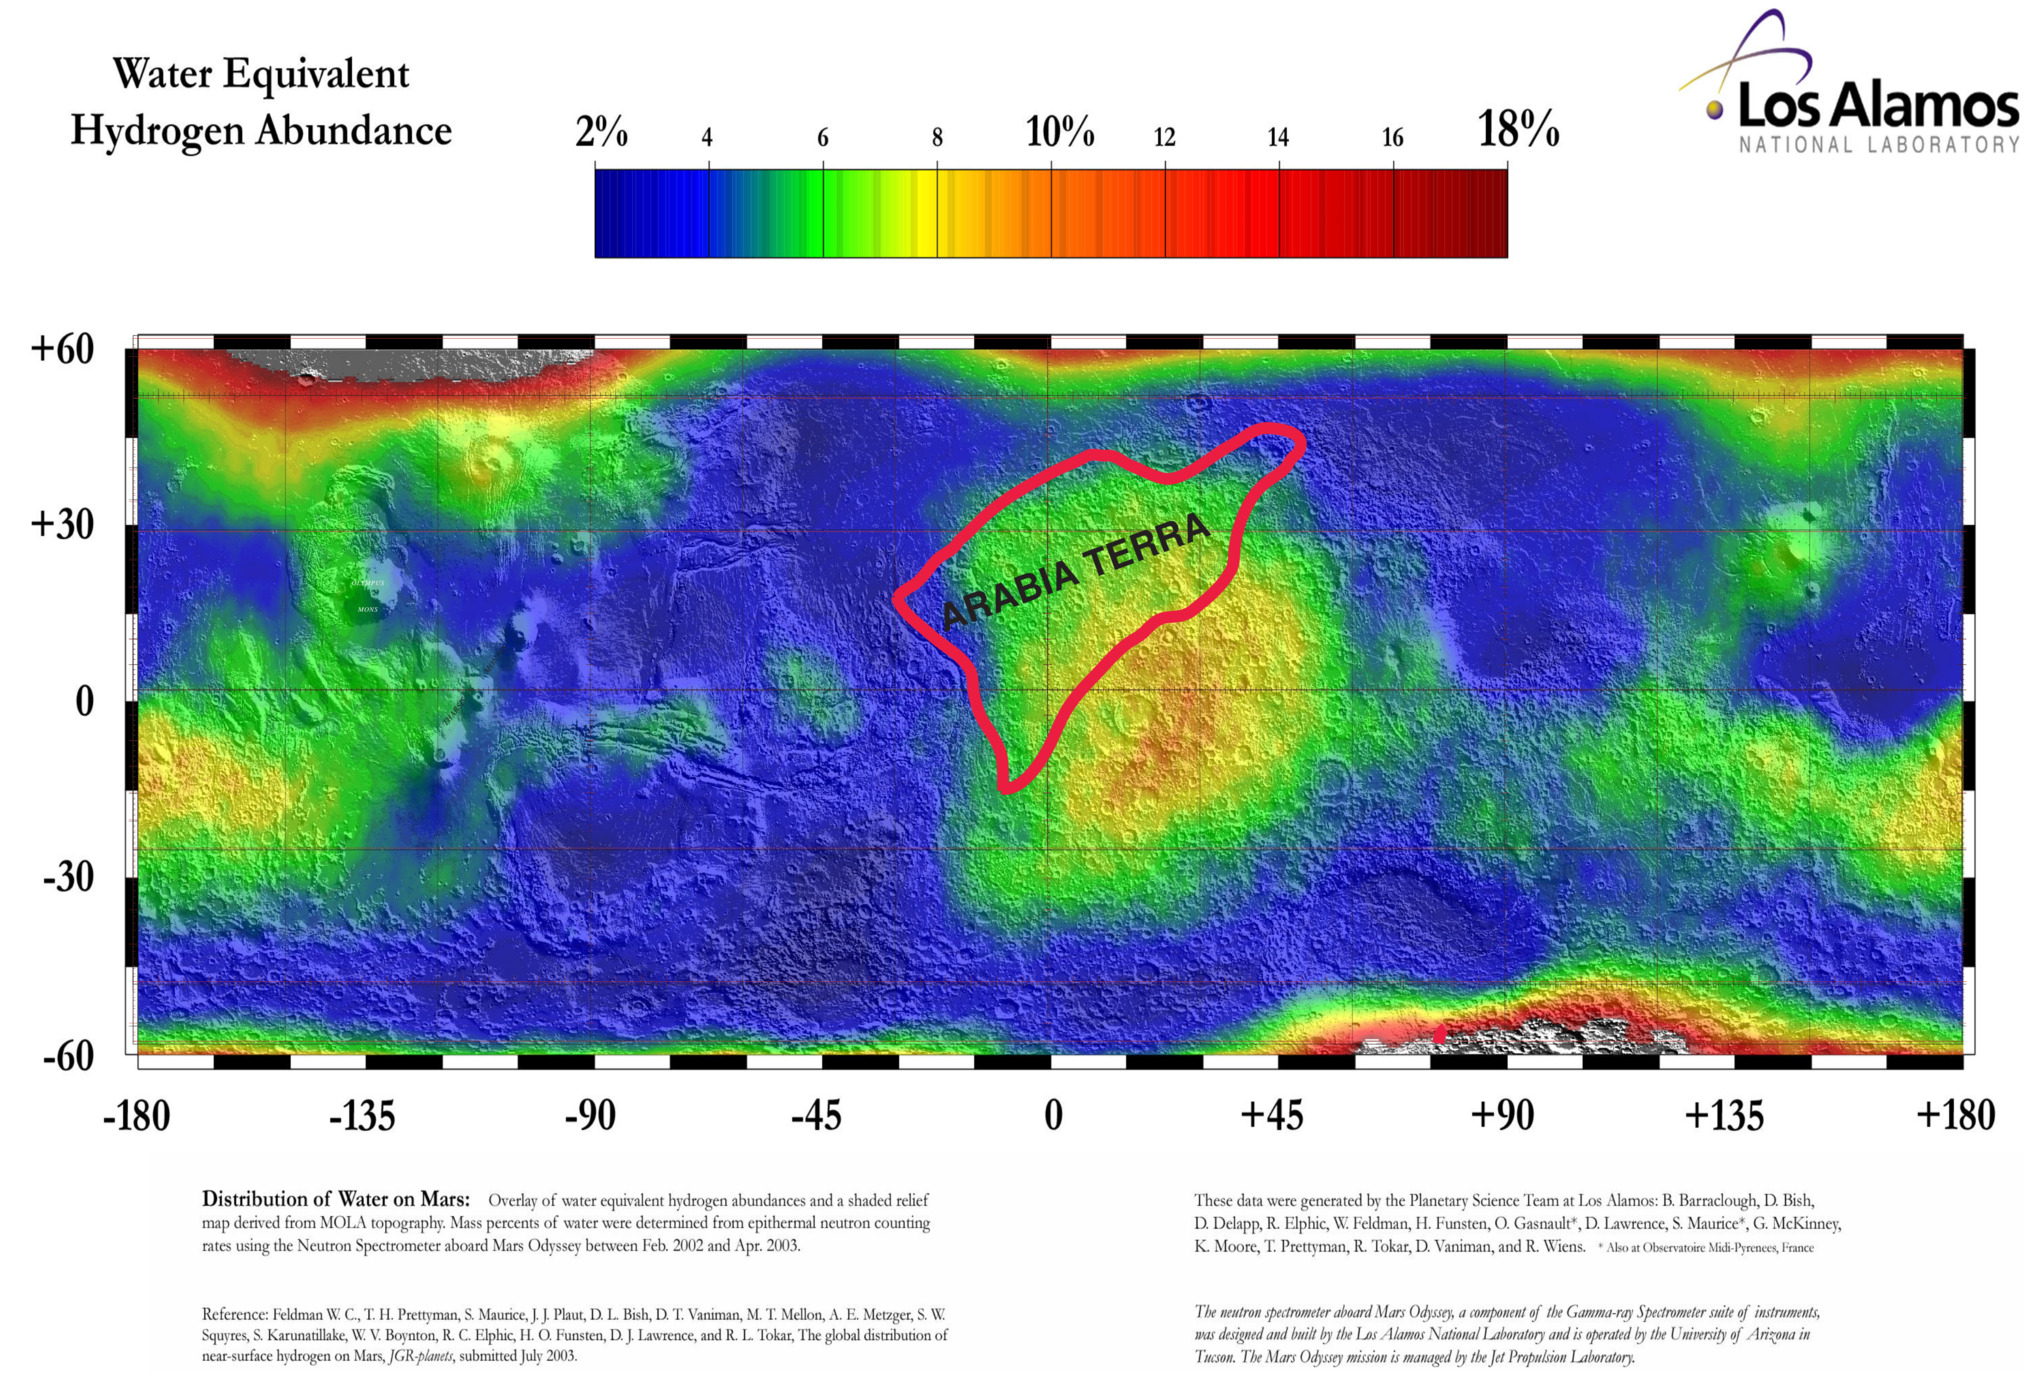
\includegraphics[width=\textwidth]{img/mola_regional_boundaries_3}
  \caption{Settlement location in Arabia Terra. The figures are modified 
versions of \cite{mars_elevation_and_boundaries} and \cite{water_on_mars}}
  \label{fig:arabia_terra}
\end{figure*}

The height varies from \SI{-4000}{\metre}weight solar panel to 
\SI{1000}{\metre} 
above the mean 
Mars surface level. In these conditions, the atmospheric pressure varies from
\SI{1001}{\pascal} to \SI{639}{\pascal}, whereas the density ranges from 
\SI{0.0212}{\kilogram\per\cubic\meter} to 
\SI{0.0138}{\kilogram\per\cubic\meter}. Although bigger pressures ensures 
better 
collection of atmospheric gases, it also reduces the operating range of the 
jet-pack as the density increases, as will be shown later.

\section{Propellant needs}

In this section we are going to calculate the amount of propellant needed to 
finish the mission safely. This amount is going to variate proportionally to 
the travel time and type of the mission, meaning that if we travel more time we 
will need more propellant and if we have a more `aggressive' mission such as 
climbing mountains or traveling at higher speed we will also need more 
propellant. 

The first stage of the problem is to enumerate the different masses of the 
system and its approximate estimation value. For this system we have:

\begin{itemize}
	\item $m_{a}$: Astronaut mass (from \SI{50}{\kilogram} to 
\SI{90}{\kilogram})
	\item $m_{e}$: Exoskeleton mass (\SI{20}{\kilogram})
	\item $m_{s}$: Suit mass (\SI{55}{\kilogram})
	\item $m_{ls}$: Life Support System mass (\SI{10}{\kilogram})
	\item $m_{es}$: Electric System mass (\SI{1}{\kilogram})
	\item $m_{\COtwo}$: Carbon dioxide mass (variable, depends on the 
propellant mass).
	\item $m_{jp}$: Jet-pack mass (\SI{30}{\kilogram})
	\item $m_{p}$: Propellant mass (from \SI{50}{\kilogram} to 
\SI{200}{\kilogram})
        \item $m_d$: Dry mass, as a sum of all the masses except the propellant 
mass.
\end{itemize} 

The rocket thrust $F$ is equal to the total weight during fixed point flight:

\begin{equation}
  F = Isp \cdot \dot{m}_p = \left( m_d + m_p \right) \cdot g
\end{equation}

\noindent where $Isp$ is the specific impulse of the rocket engine and 
$\dot{m}_p$ is the propellant mass flow rate. This specific impulse has been 
computed for different altitudes, from \SI{-4000}{\metre} to \SI{1000}{\metre}, 
and for a combustion chamber pressure going from \SI{10}{\mega\pascal} to 
\SI{50}{\mega\pascal}. \autoref{fig:isp} shows the results for the specific 
impulse computed using CEA \cite{cea}. The specific impulse seems to be bigger 
than \SI{3000}{\metre\per\second} until the combustion chamber pressure drops 
to values close to \SI{10}{\mega\pascal}. Also, its value starts to decrease in 
a dramatic way as this pressure becomes smaller, so a minimum combustion 
chamber pressure of \SI{10}{\mega\pascal} will be imposed.

\autoref{fig:T} shows the jet outlet temperature at different altitudes and 
combustion chamber pressures. The values are relatively cold, reducing the risk 
for the astronaut. The combustion chamber temperature ranges from 
\SI{1290}{\kelvin} to \SI{1440}{\kelvin}, so the walls will be cooled down 
using the liquid oxidant and fuel.

\begin{figure*}
  \centering
  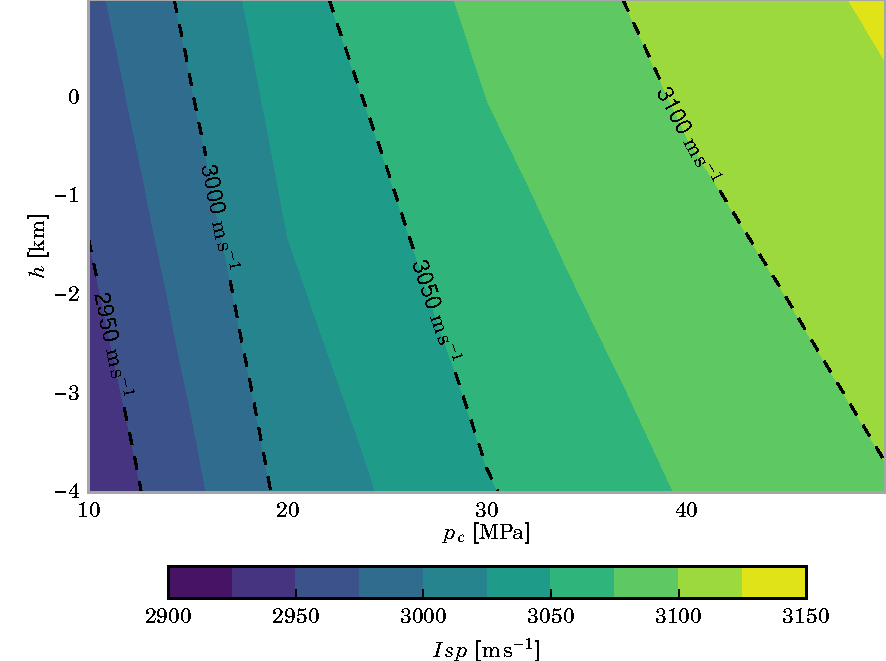
\includegraphics{img/isp}
  \caption{Specific impulse for different combustion chamber and ambient 
pressures}
  \label{fig:isp}
\end{figure*}

\begin{figure*}
  \centering
  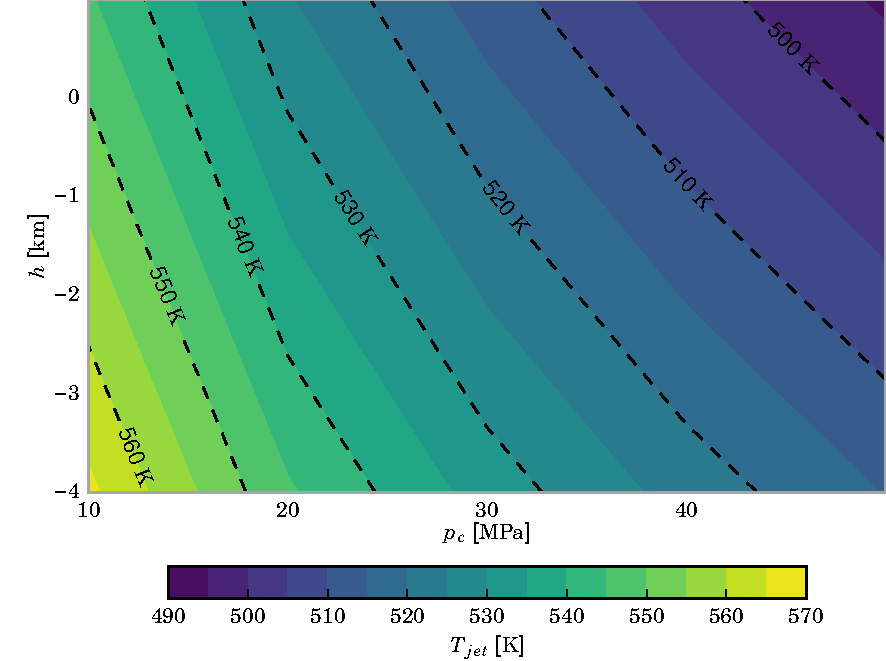
\includegraphics{img/T}
  \caption{Specific impulse for different combustion chamber and ambient 
pressures}
  \label{fig:T}
\end{figure*}

$\COtwo$ is needed to pressurize the fuel and oxidizer, and is a function of 
the total mass of them. This mass will be set as the one needed to keep the 
combustion chamber pressure bigger than \SI{10}{\mega\pascal}. To reduce the 
performance reduction due to $\COtwo$ diffusion in the fuel or the oxidant, a 
piston should be used. Results for the mass of $COtwo$ needed are shown in 
\autoref{fig:co2}: around of one third of the propellant mass will be 
needed in $COtwo$ mass for pressurization. Also, a 
turbopump might be used for pressurization instead of $\COtwo$: it has the 
advantage of a smaller weight, but it is more complex and complicated to 
maintain.

In this fixed-point flight mission, the jet-pack endurance is:

\begin{equation}
  \Delta t = -\int_{{m_p}_0}^0 \cfrac{Isp \ud m_p}{g \cdot \left( m_d + m_p 
\right)} = \ln{\cfrac{m_d + m_p}{m_d}}
\end{equation}

\autoref{fig:delta_t_co2} shows the jet pack operating time for propellant 
masses ranging from \SI{50}{\kilogram} to \SI{200}{\kilogram} and astronaut 
masses from \SI{50}{\kilogram} to \SI{90}{\kilogram}, using $\COtwo$ for 
pressurization. \autoref{fig:delta_t_co2} shows the same information, using a 
turbopump of \SI{10}{\kilogram}. A propellant mass of \SI{100}{\kilogram} 
ensures more than \SI{300}{\second} of operation in either case for the whole 
range of astronaut mass. A propellant mass of \SI{100}{\kilogram} and a 
$\COtwo$ 
pressurization system is selected to reduce the complexity of the system. The 
total mass is around \SI{350}{\kilogram} and, even in the reduced gravity of 
Mars' surface, this produces a weight equivalent to that of \SI{132}{\kilogram} 
in Earth. Even more, the total momentum is big enough to produce a lot of 
problems for the astronaut to move around freely. An exoskeleton is added to 
reduce these problems, increasing the astronaut's force. The exoskeleton 
introduces also an extra layer of protection against physical accidents, 
increasing the safety of the mission.

\begin{figure*}
  \centering
  \begin{subfigure}{\textwidth}
    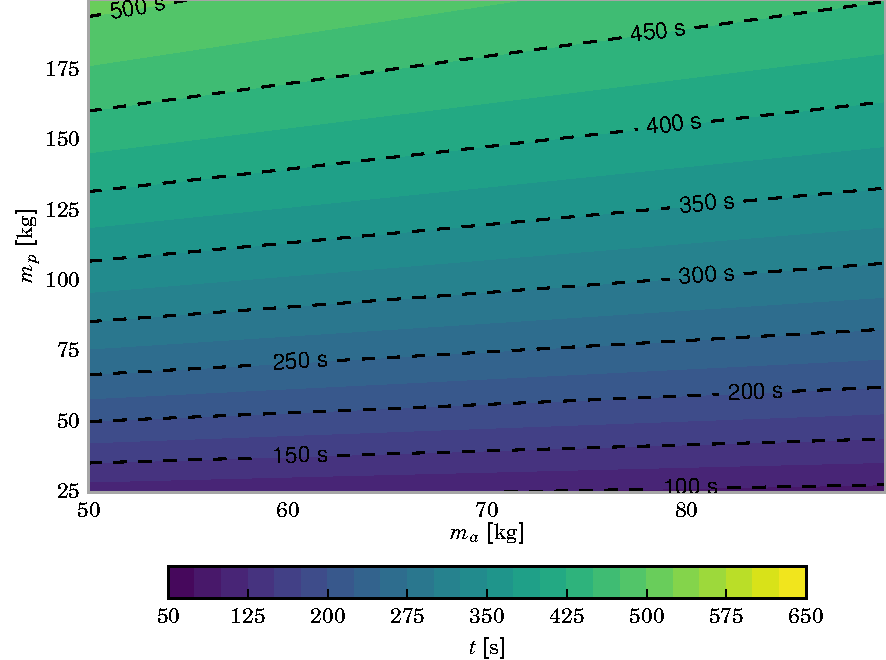
\includegraphics{img/delta_t_co2}
  \caption{Jet-pack operating time for different propellant and astronaut 
  masses, using $\COtwo$ for pressurization.}
    \label{fig:delta_t_co2}
  \end{subfigure}
  \begin{subfigure}{\textwidth}
    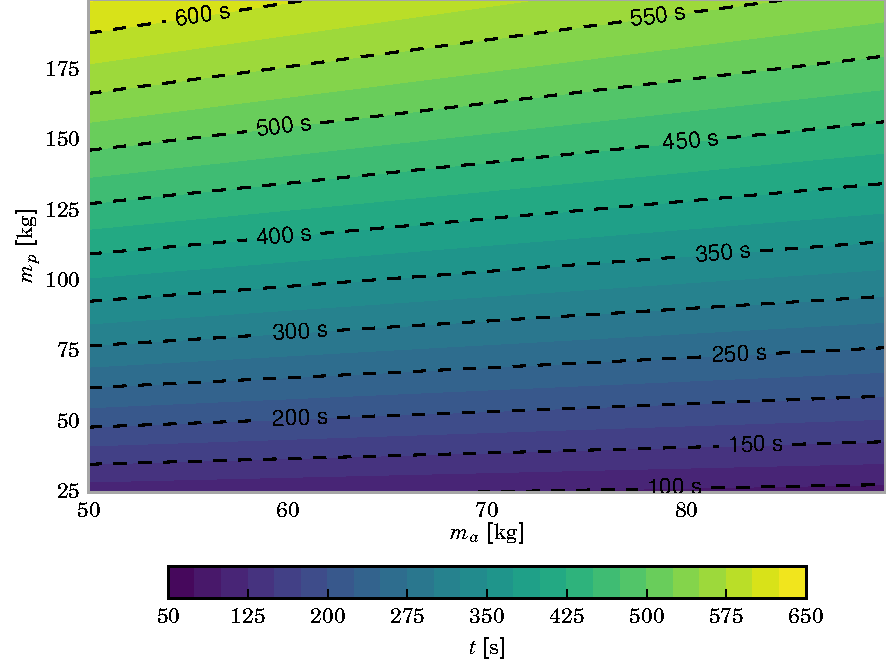
\includegraphics{img/delta_t_tp}
  \caption{Jet-pack operating time for different propellant and astronaut 
  masses, using a turbopump for pressurization.}
    \label{fig:delta_t_tp}
  \end{subfigure}
\end{figure*}

\begin{figure}[h]
  \centering
  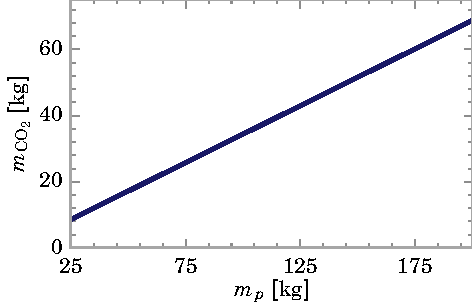
\includegraphics{img/co2}
  \caption{$\COtwo$ mass needed for pressurization as a function of the 
propellant mass}
  \label{fig:co2}
\end{figure}


\section{Maximum horizontal range}

In the following figures, the maximum horizontal range for jet-pack operation 
is shown. In this case, the total thrust $Isp \cdot \dot{m}_p$ when the 
steady-state speed is reached is:

\begin{equation}
  Isp \cdot \dot{m}_p
  =
  \sqrt{\left(\cfrac{1}{2} \cdot \rho \cdot v^2 \cdot A_f \cdot C_D\right) ^ 2
  + \left[ \left( m_d + m_p \right) \cdot g \right] ^ 2}
\end{equation}

\noindent where $A_f$ is the frontal area, equal to around 
\SI{2}{\meter\squared}, $C_D$ is the drag coefficient, equal to $1.3$, 
and $v$ is the flow speed.

The flight endurance is:

\begin{equation}
  t = \left. \cfrac{2 \cdot Isp \cdot
  \tan^{-1}{
\frac{8 \cdot g ^ 2 \cdot m_p + 8 \cdot g ^ 2 \cdot m_d}
{4 \cdot A_f \cdot C_D \cdot g \cdot \rho \cdot v^2}
}}
  {A_f \cdot C_D \cdot g \cdot \rho \cdot v^2}
  \right|_{{m_p}_0}^{{m_p}_1}
\end{equation}

\noindent where ${m_p}_0$ is the initial propellant mass, equal to
\SI{95}{\kilogram}, and ${m_p}_1$ is the final propellant mass, equal to 
\SI{5}{\kilogram}. Around \SI{10}{\kilogram} of propellant are not used during 
this steady-state phase: it will be used for take-off, acceleration, 
deceleration and landing. The range is, thus:

\begin{equation}
  L = t \cdot v
\end{equation}

\autoref{fig:l_ma_60} shows the mission range for a \SI{60}{\kilogram} 
astronaut, whereas \autoref{fig:l_ma_90} shows the same information for a 
\SI{90}{\kilogram} astronaut. The figures show optimum speeds for different 
altitudes: this optimum speed grows with rising altitudes and ranges between 
\SI{175}{\metre\per\second} to slightly more than \SI{210}{\metre\per\second}. 
The maximum range is obtained for the maximum altitude, being more than 
\SI{35}{\kilo\metre}. When using a propellant mass of \SI{25}{\kilogram}, the 
range is greatly reduced, but is still enough for more than 
\SI{6.5}{\kilo\metre} missions, as shown in \autoref{fig:l_ma_60_mp_25} and 
\autoref{fig:l_ma_90_mp_25}.

\begin{figure*}[h!]
  \centering
  \begin{subfigure}{\textwidth}
    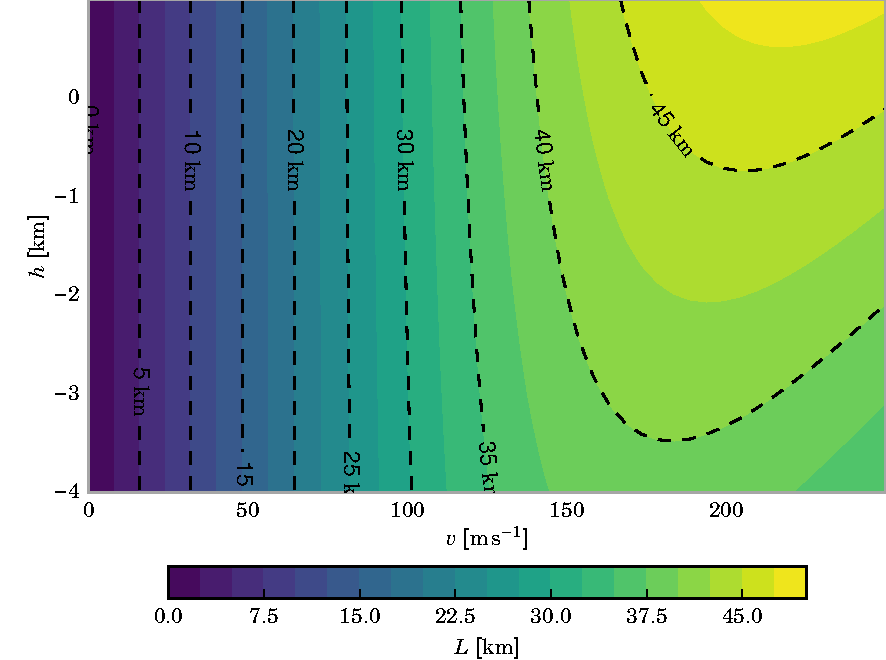
\includegraphics{img/l_ma_60}
  \caption{Jet-pack endurance at different altitudes and speeds, for an 
astronaut mass of \SI{60}{\kilogram}, \SI{100}{\kilogram} of propellant
and using $\COtwo$ for pressurization.}
    \label{fig:l_ma_60}
  \end{subfigure}
  \begin{subfigure}{\textwidth}
    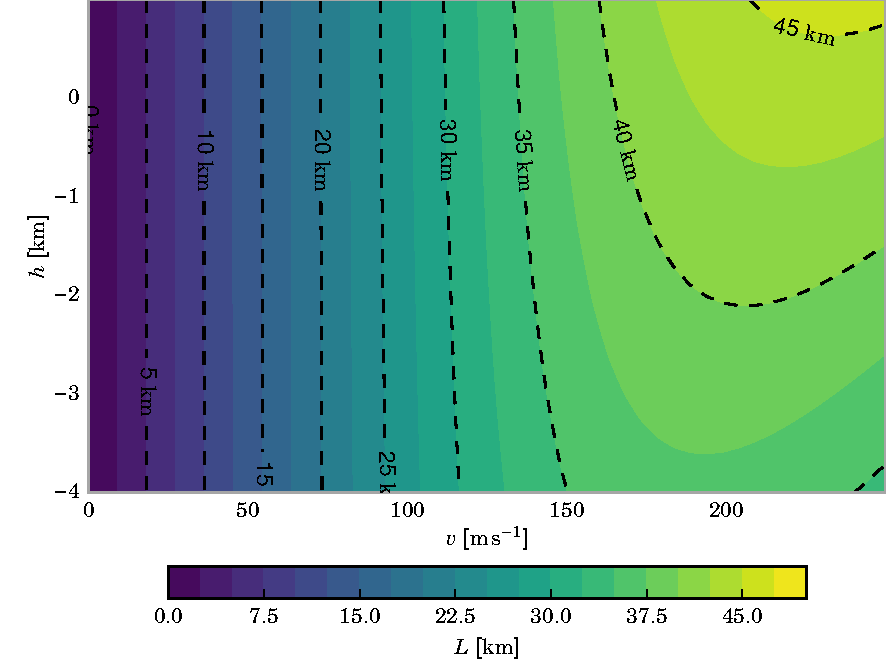
\includegraphics{img/l_ma_90}
  \caption{Jet-pack endurance at different altitudes and speeds, for an 
astronaut mass of \SI{90}{\kilogram}, \SI{100}{\kilogram} of propellant
and using $\COtwo$ for pressurization.}
    \label{fig:l_ma_90}
  \end{subfigure}
\end{figure*}

\begin{figure*}[h!]
  \centering
  \begin{subfigure}{\textwidth}
    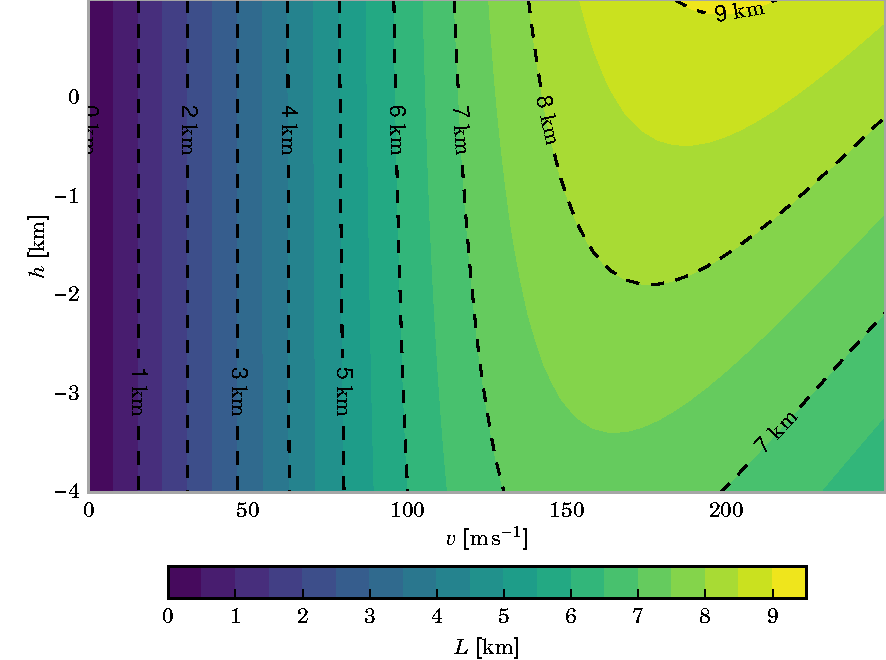
\includegraphics{img/l_ma_60_mp_25}
  \caption{Jet-pack endurance at different altitudes and speeds, for an 
astronaut mass of \SI{60}{\kilogram}, \SI{25}{\kilogram} of propellant
and using $\COtwo$ for pressurization.}
    \label{fig:l_ma_60_mp_25}
  \end{subfigure}
  \begin{subfigure}{\textwidth}
    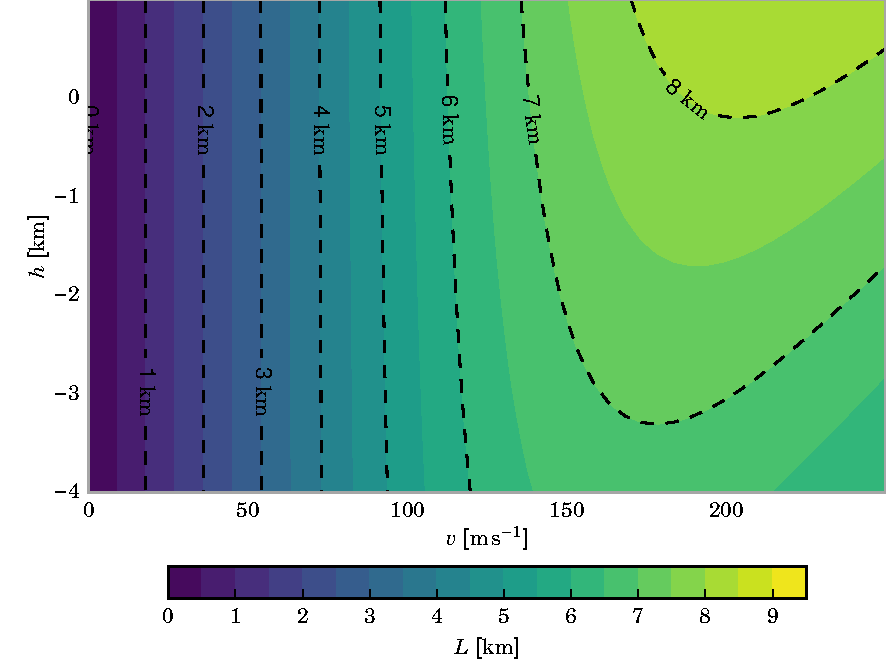
\includegraphics{img/l_ma_90_mp_25}
  \caption{Jet-pack endurance at different altitudes and speeds, for an 
astronaut mass of \SI{90}{\kilogram}, \SI{25}{\kilogram} of propellant
and using $\COtwo$ for pressurization.}
    \label{fig:l_ma_90_mp_25}
  \end{subfigure}
\end{figure*}
\section{Jet-pack architecture}

Having discussed the feasibility of the system it is necessary to tackle its 
physical layout. It has been decided to design the jet-pack so the bulk of the 
astronaut mass and propellant mass swings below the propulsion nozzles. This 
way, the natural stability of the system means that no active control is needed 
on this axis. Several designs were studied and it was concluded that the one 
that minimizes weight while keeping the system safe and controllable is a twin 
nozzle configuration side to side across the user's shoulders.
A pair of actuated gimbaled nozzles is going to be mounted on a foldable cross 
member. When the system is unused it can be retracted on the back of the 
wearer, re-opening again when needed. A specific mechanical hinge will ensure 
that the open position is the one of maximum strength by limiting the range of 
movement of the aforementioned hinge.
The gimballing action of the nozzles provides active yaw, lateral, longitudinal 
and translation control capabilities. The actuators for this system will be 
electromechanical in order to keep a low weight figure. Roll and pitch control 
are passively stable due to the configuration elected and, since the martian 
atmosphere is very thin, there is no important impact on flight performance due 
to poor aerodynamic astronaut flying position. Also, it is desirable to use 
aerospike type nozzles to accommodate for change in pressure conditions while 
using the jet-pack on different scenarios and maximize the specific impulse of 
the rocket engines while keeping the weight low efficiently.
\autoref{fig:concept_art} shows a concept for the jet-pack physical appearance 
together with the exoskeleton.

\section{Exoskeleton description}

As it has been described along this work, the astronaut will be carrying over 
three times its mass during the development of an EVA. Despite the martian 
gravity is roughly a third of Earth's, the inertia of this increased mass means 
that the stability of the astronaut and its dexterity performing tasks will me 
diminished. To avoid potentially dangerous situations, muscular fatigue and to 
increase the versatility of the mission, the proposed transport solutions 
relies on the use of an exoskeleton.

This exoskeleton shall be worn on top of a EVA suit and it should be able to 
be removed and equipped by a single astronaut. This can be accomplished if the 
suit is setup as a chair (in a metaphorical sense) that embraces its carrier.
The suit will augment the force and dexterity of the user via electromyographic 
sensing and positive feedback on intelligent polymer fabrics and actuators. 
These polymers will contract and relax through current applications, imitating 
the natural muscle workings.
Fully sensored, it will be able to monitor the user's overall health status, 
report medical conditions to the mothership and it could even serve as a 
resuscitation aid should a cardiac arrest occur. Also, it could provide aid in 
the rehabilitation of lesions and ease the transport of injured personnel 
through immobilization of the patient or its injured member, joint or zone.

The field of intelligent polymers and fabrics has experienced a steady growth 
in the last decade. Today, many materials are capable of altering their 
mechanical, optical, electrical and surface properties in response to different 
stimuli. These materials range from electric field sensitive  fabrics to 
magnetic field dependent composites and fluids. The proposed exoskeleton would 
make use of these technologies in order to provide both support and strength to 
the wearer.
%Concepts here
% Sketches and concept illustrations for the proposed system are shown in figures 
% .
With the current technology, this system would allow a regular astronaut, which 
would have lost an important part of his muscle due to microgravity during the 
travel, to perform tasks safely and effectively, maximizing the travel's 
scientific throughput.

\section{Augmented reality system}

The transport solution here developed entitles not only the jet-pack and the 
exo-suit, but a complex augmented reality HUD helmet and system. The user of 
the suit will have available a customizable selection of several parameters of 
the environment and its suit. This information will be presented through an 
immersive Heads-Up-Display that will react and learn with the user, a concept 
for the helmet is shown in figure \autoref{fig:casco_art}.
The data captured by the sensors of the suit will be processed and relayed to 
other astronauts and the exploration base for further analysis. Additionally, 
our design incorporates a bracelet which can be used to monitor key health 
parameters and the status of the suit's systems. This is not just used for the 
visualization of the main user, but also for other astronauts to aid in case of 
depressurization, accident or other kinds of dangerous situations.

\section{Connectivity and systems integration}

The suit's systems will interact together with the jet-pack controls and 
processing units. It is key to provide advanced functionality besides the basic 
flight capability. A selection of different selected features would be:
\begin{itemize}
	\item Health monitoring: As mentioned, the suit will interact with the 
user and it will be able to measure key vital parameters and other information 
such as load bearing on joints and limbs or provide an interface with the 
user's brain functions via non-intrusive electroencephalography or other kinds 
of BMIs. Eye-tracking technology will be incorporated so the user can aid the 
exploration of the environment by the suit's sensor set.
	\item Navigation: It is key to the augmented reality system to be able 
to show real-world and real-time information about the topography, relief, 
distance, composition and any other relevant known fact of the terrain to the 
user. This function together with the ability to enable users to mark key 
waypoints and information would enable fast and responsive exploration events.
	\item Threat alert: Weather forecasting and potentially dangerous 
terrain alerts shall be part of a threat alert system for the HUD.
	\item Automatic flight: Despite it will be piloted normally for 
flights, it is possible to include autonomous flight capabilities to the system. 
This would allow the user to demand a suit in certain situations and it would be 
able to fly towards the user or return to the base for autonomous recharging.
	\item Terrain recognition: It is interesting to obtain high resolution 
martian scanning data while the jet-pack is flying. It provides an opportunity 
to mount a stereoscopic camera to t and perform these scans on-the-fly.
\end{itemize}

\section{Mission concept}

This development, although very interesting from the perspective of Mars 
exploration, would require a mass budget that makes it difficult for being 
included on a crewed mission, specially the fuel processing equipment. To aid 
with this, a sequential mission is proposed. Firstly, a set of supply missions 
would be launched from the Earth during a Mars transfer window. These missions 
would transport the habitat for the explorers as well as supplies for the 
mission and an RTG-powered robotic fuel processing factory. This factory would 
have arrived to the planet with sufficient time in order to process the 
required amounts of products in order to generate the fuel, not just for the 
jet-pack, but possibly for enabling the return vehicle to carry a greater 
payload back to Earth.
As the factory would slowly produce methane and oxygen from the martian soil 
and atmosphere it will also extract other components such as surplus water for 
the mission, Argon, Carbon dioxide, pure Carbon, Magnesium, Aluminum, Silicon, 
Phosphorus, Chlorine, Sulfur, Calcium, Titanium, Iron and other metal amounts. 
Using these, a set of replicating factories could be built and an expanding 
robot based exploration could be started, easing future exploration and 
colonies. Further power needs will be supplied with later solar panel upgrades.

\begin{figure*}
  \centering
    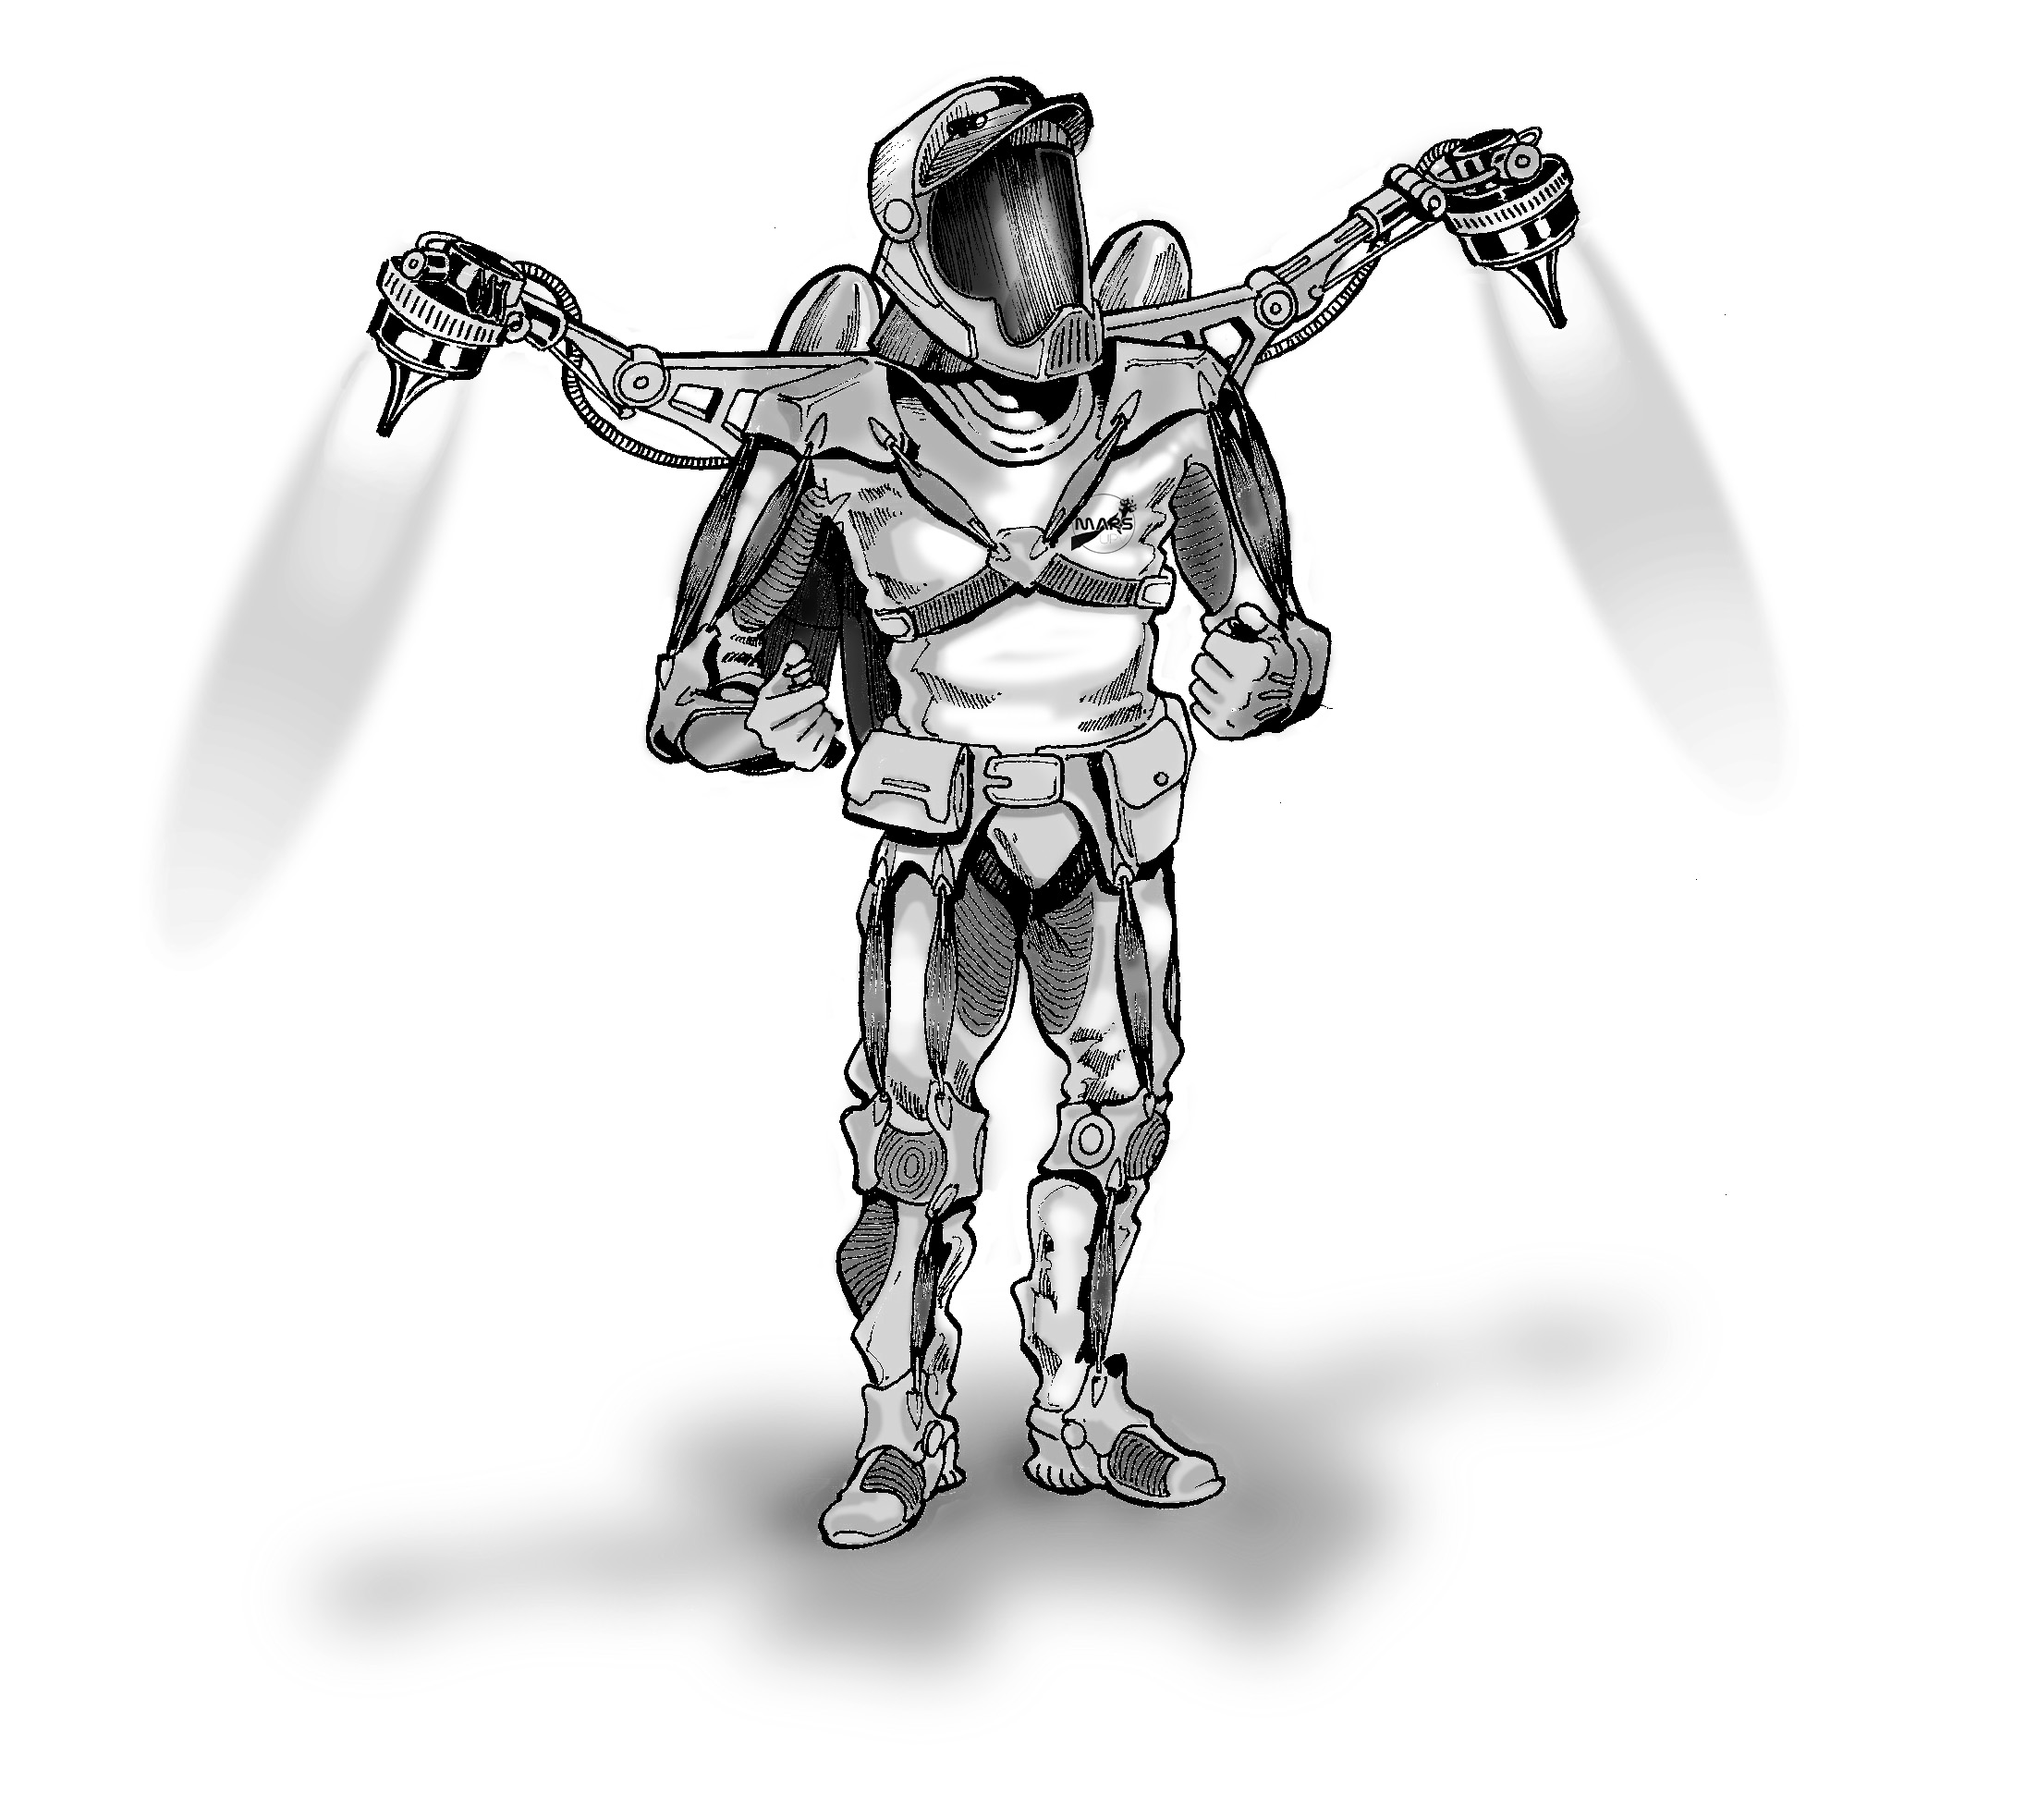
\includegraphics[width=\textwidth]{img/frontal_v2.jpg}
  \caption{Jet-pack concept art.}
    \label{fig:concept_art}
\end{figure*}

\begin{figure*}
  \centering
    \includegraphics[width=\textwidth]{img/01_casco.jpg}
    \caption{HUD helmet concept art.}
    \label{fig:casco_art}
\end{figure*}

\section{Conclusions}

A LOX + $\CHfour$ powered jet-pack is proposed to ease early human settlements 
on Mars. This jet-pack can be used as a mobility solution, enabling the 
astronauts to fly over obstacles and to move fast between different outposts.

\SI{100}{\kilogram} of propellant ensures more than \SI{300}{\second} of 
fixed-point operation and more than \SI{35}{\kilo\metre} of horizontal range at 
high speeds. The production of the propellant can be easily done using water 
from the ground and atmospheric $\COtwo$ and a moderate surface of solar cells 
for producing electrical energy.

An exoskeleton is also used to increase the astronaut's force, as the total 
mass of the system plus astronaut can be around \SI{350}{\kilogram} when fully 
loaded with fuel. The exoskeleton is even interesting as an extra layer of 
protection against physical harm and can provide extra functionality.

\section*{List of symbols}

\begin{table}[H]
  \centering
  \begin{tabular}{cc}
    \toprule
    Symbol & Description \\
    \midrule
    $A_f$ & Frontal area \\
    $C_D$ & Drag coefficient \\
    $F$ & Thrust \\
    $g$ & Acceleration of gravity \\
    $h$ & Altitude \\
    $Isp$ & Specific impulse \\
    $L$ & Range \\
    LOX & Liquid oxygen \\
    $m_a$ & Astronaut mass \\
    $m_{\COtwo}$ & Mass of $\COtwo$ \\
    $m_d$ & Dry mass \\
    $m_e$ & Exoskeleton mass \\
    $m_{es}$ & Electric system mass \\
    $m_{jp}$ & Jet-pack mass \\
    $m_{ls}$ & Life support mass \\
    $m_p$ & Mass of propellant \\
    $m_s$ & Suit mass \\
    $\dot{m}_p$ & Propellant mass flow \\
    $\rho$ & Atmospheric density \\
    $t$ & Time \\
    $T$ & Temperature \\
    $v$ & Flight speed \\
    \bottomrule
  \end{tabular}
\end{table}


\printbibliography

\end{document}